\documentclass[12pt,a4paper]{article}

% Margins.
\setlength{\oddsidemargin}{0in}
\setlength{\evensidemargin}{0in}
\setlength{\headheight}{12pt}
\setlength{\headsep}{0pt}
\setlength{\topmargin}{-60pt}
\setlength{\textwidth}{6.5in}
\setlength{\textheight}{10.75in}

\usepackage{amsmath}
\usepackage{float}
\usepackage{graphicx}
\usepackage[hyphens]{url}
\usepackage{hyperref}	% Clickable links to figures, references and urls.
\usepackage{datetime}
\usepackage{longtable}

% Drawing.
\usepackage{pgf}
\usepackage{tikz}

% Listings for formatting code.
\usepackage{listings}
\usepackage{textcomp}
% General options.
\lstset{breaklines=true, basicstyle=\small\ttfamily, tabsize=4, numbers=left, stepnumber=1, frame=single, showstringspaces=false, upquote=true}
% C++ specific high-lighting. Comments are 50/50 shades of green/black and strings coloured with 60/40 red/black mixture.
\lstset{language=[ISO]C++, commentstyle=\color{green!50!black}, keywordstyle=\color{blue}, stringstyle=\color{red!60!black}}

%opening
\title{Electromagnetic Theory\\Class 01\\Introduction\\Scalars and Vectors}
\author{Attique Dawood}
\date{August 25, 2014\\[0.2cm] Last Modified: \today, \currenttime}
\begin{document}
\maketitle
\section{About the Course}
\textbf{Course Title:} Electromagnetic Theory\\
\textbf{Course Code:} NS110\\
\textbf{Pre-requisite(s):} Physics for Engineers, Multi--variable Calculus/CVT\\
\textbf{Credit Hrs:} 3\\
\textbf{Instructor:} Attique Dawood\\
\textbf{Contact:} attique DOT dawood AT nu DOT edu DOT pk\\
\section{Text Book}
\textbf{Title:} Elements of Electromagnetics (3$^{rd}$ Edition)\\
\textbf{Author:} M. N. O. Sadiku\\
\section{Objective}
The objective of this course is to introduce the basics of electromagnetics. Emphasis is on mathematically solving problems involving electric and magnetic fields. After taking this course students will be familiar with Maxwell’s equations and will be able to solve problems related to electrostatics and magnetostatics.
\section{Guidelines}
\begin{itemize}
\item \textbf{\underline{Your must do all assignments by yourself.}}
\item You can only learn with practice.
\end{itemize}
\section{Marks Distribution}
\begin{table}[H]
\begin{center}
\vspace{0.3cm}
	\begin{tabular}{llc}
	\hline \hline
		\rule{0pt}{2.6ex} & \textbf{Type of Assessment} & \textbf{Marks}\\
		\hline
		1 \rule{0pt}{2.6ex} & Quizzes & 10\\
		2 & Assignments& 10\\
		3 & Sessionals (15 each) & 30\\
		4 & Final Exam & 50\\
	\hline \hline
	\rule{0pt}{2.6ex} & \textbf{Total} & \textbf{100}\\
	\hline \hline
	\end{tabular}
\end{center}
\label{Marks Distribution}
\caption{Marks Distribution}
\end{table}
\section{Course Contents}
Course outline is available on SLATE.
\section{Advertisement}
This section is taken from \cite{Griffith}.
\begin{itemize}
	\item[1.] \textbf{What is \textit{Change}?} Changes are happening all around us; from a car running on the road, a person talking, people walking, earth revolving around the sun to vibration of atoms in matter.
	\item[2.] \textbf{What would happen if there were no change and all the atoms in the universe are frozen?} Nothing, everything will stop and all activities will come to a standstill. Heat death?
	\item[3.] \textbf{What causes Change?} Force.
\end{itemize}
Behind every change there is a force. We see different forces at work in everyday life; we can push a chair or object by applying a force, we can lift objects by applying a force and so on. \textit{Mechanics} is concerned with forces and changes they cause. You will be surprised to know that in the realm of physics there are only four known forces. These are listed below in the order of decreasing strength:
\begin{enumerate}
\item Strong. (keeps protons and neutrons bound in nucleus)
\item Electromagnetic.
\item Weak. (responsible for radioactive decay)
\item Gravitational.
\end{enumerate}
You might ask where is friction, or normal force or chemical forces that bind molecules. The answer is that all of these forces are electromagnetic. We do not feel strong or weak forces because they have a very short range and confined to nucleus of atom. Gravity is so weak that we can only notice it for large objects with huge masses like sun or earth. \textbf{``Not only are electromagnetic forces overwhelmingly the dominant ones in everyday life, they are also, at present, the \textit{only} ones that are completely understood.''}\cite[page 14]{Griffith}

``The Laws of classical electrodynamics were discovered in bits and pieces by Franklin, Coulomb, Ampere, Faraday and others.'' It was Maxwell who combined all these Laws in the current form, called Maxwell's equations.

\textbf{Our goal in this course is to get an understanding of how electrodynamics work by studying the Maxwell's equations.} But knowing how Maxwell's equations work is not the end, this is only the beginning where you will start applying these fundamental laws and equations to solve larger problems. In the later part of this course we will use Maxwell's equations to explore how electromagnetic waves propagate in space.

\section{Engineering and Scientific Notations}
\subsection{A Note on Scientific Notation}
You should already be familiar with scientific notation which is of the form $1.234\times10^3$ or $-3.2343\times 10^{-4}$ etc. Scientific notation is essentially a number greater than 0 and less than 10 with appropriate sign multiplied with power of 10. An alternate form of scientific notation commonly used in computers and calculators, replaces $\times 10$ with `e' or `E'. For example, $1.234\mathrm{e}3$ and $-3.2343\mathrm{e}$$-4$. You can access this on your calculator with the `Exp' key.
\subsection{Engineering Notation}
A number expressed in engineering notation consists of a numerical part with an appropriate symbol representing power of 10. The numerical part is greater than 1 and less than 1000 with appropriate sign. Working with engineering notations is generally preferred because of ease of use. A table of engineering symbols is given below.
\begin{table}[H]
\begin{center}
	\begin{tabular}{|c|c|c||c|c|c|}
	\hline \hline
		%\rule{0pt}{2.6ex} \textbf{Week} & \textbf{Topics}\\
		%\hline
		k\rule{0pt}{2.6ex} & kilo & $10^3$ & m & milli & $10^{-3}$\\
		M & mega & $10^6$ & $\mu$ & micro & $10^{-6}$\\
		G & giga & $10^9$ & n & nano & $10^{-9}$\\
		T & tera & $10^{12}$ & p & pico & $10^{-12}$\\
		P & peta & $10^{15}$ & f & femto & $10^{-15}$\\
		E & exa & $10^{18}$ & a & atto & $10^{-18}$\\
	\hline \hline
	%\label{Engineering-symbols}
	%\caption{Physics for Engineers Course Outline}
	\end{tabular}
\end{center}
\label{Engineering-symbols}
\caption{Engineering symbols}
\end{table}
\noindent In engineering notation, $1.234\times10^3$ is written as $1.234k$ and $-3.2343\times 10^{-4}$ as $-323.43\mu$.
\section{Exercises}
\noindent\textbf{Question 1:} How much distance does light travel in one year? Speed of light is $3\mathrm{e}8$ m/s.\\
\noindent\textbf{Question 2:} Express the following speeds in m/s:\\
\begin{enumerate}
\item[-] 19 km/h
\item[-] 0.030 mi/h
\item[-] 1.9 km/min
\item[-] 1000 cm/s
\item[-] 1900 km/day
\end{enumerate}
Perform all calculations in engineering notation.
\subsection{Scalars}
A scalar quantity has only magnitude. Distance, mass, time, etc. are examples of some scalars. A scalar quantity is represented by a plain letter, e.g, $A, t, m$.
\subsection{Vectors}
Vector quantities require a direction along with magnitude. If you want directions to the nearest restaurant and ask someone, you get an answer like this: ``Walk a distance of 100 m and you'll get there.'' Does this make any sense? You know how much distance you have to travel but you don't know which direction to go! Instead if you are told: ``Walk 100 m westward.'' This gives a complete description of where your destination is. Some examples of vectors are displacement, velocity, force, electric field, etc.

A vector quantity is represented by boldface (capital) letter or a letter with a bar or arrow above. Unit  vectors are usually represented with small boldface letters or with a hat above. Examples of vector notation are: $\textbf{{A}}, \vec{A}, \bar{A}, \textbf{x}, \hat{x}$.

Boldface notation is usually used in printed text. It is easier to use a bar for vectors in hand--written text.
\section{Unit Vector (1.4S)}
A vector \textbf{A} has both magnitude and direction. The \textit{magnitude} of vector \textbf{A} is a scalar quantity written as $A$ or $|\textbf{A}|$. A \textit{unit vector} $\hat{a}_A$ along \textbf{A} is defined as a vector that has the same direction as \textbf{A} but a magnitude of 1.
\begin{equation}
\hat{a}_A=\dfrac{\textbf{A}}{|\textbf{A}|}=\dfrac{\textbf{A}}{A}
\end{equation}
Note that $|\hat{a}_A|=1$. Vector \textbf{A} can be written as,
\begin{equation}
\textbf{A}=A\hat{a}_A
\end{equation}
\section{Representation of Vectors in Cartesian Coordinate System}
A vector \textbf{A} in Cartesian coordinate system is written as,
\begin{equation}
(A_x,A_y,A_z)~or~\textbf{A}=A_x\hat{x}+A_y\hat{y}+A_z\hat{z}
\end{equation}
$A_x$, $A_y$ and $A_z$ are called \textit{components} of \textbf{A} in $x$, $y$ and $z$ directions, respectively. The unit vectors $\hat x$, $\hat y$ and $\hat z$ point in the increasing direction of $x$, $y$, and $z$.
\begin{figure}[H]
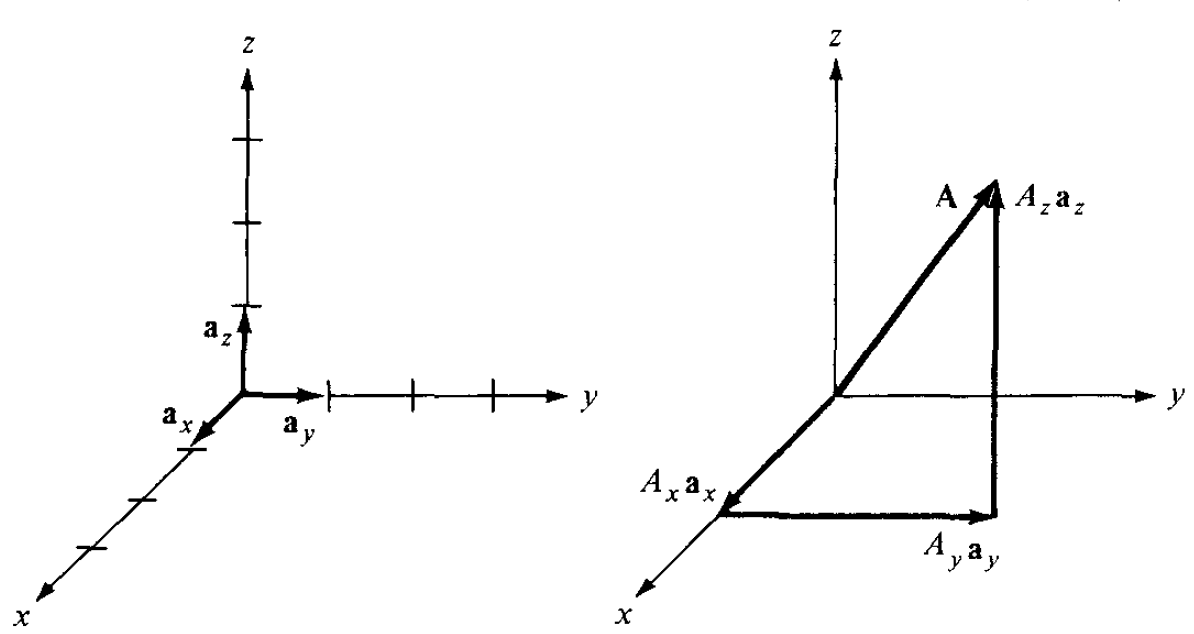
\includegraphics[scale=0.5]{Figure1-1S.png}
\caption{Representation of a vector in Cartesian coordinates \cite[fig. 1.1]{Sadiku}}
\label{components-of-A}
\end{figure}
The magnitude of \textbf{A} is given by,
\begin{equation}
|\textbf{A}|=A=\sqrt{A_x^2+A_y^2+A_z^2}
\end{equation}
The unit vector along \textbf{A} is given by,
\begin{equation}
\hat{a}_A=\dfrac{\textbf{A}}{A}=\dfrac{A_x\hat{x}+A_y\hat{y}+A_z\hat{z}}{\sqrt{A_x^2+A_y^2+A_z^2}}
\end{equation}
\section{Addition and Subtraction of Vectors (1.5S)}
Vectors \textbf{A} and \textbf{B} can be added together to give a third vector \textbf{C},
\begin{equation}
\textbf{C}=\textbf{A}+\textbf{B}
\end{equation}
If $\textbf{A}=(A_x,A_y,A_z)$ and $\textbf{B}=(B_x,B_y,B_z)$ then,
\begin{equation}
\textbf{C}=(A_x+B_x)\hat x+(A_y+B_y)\hat y+(A_z+B_z)\hat z
\end{equation}
Vector subtraction is carried out in a similar manner.
\begin{equation}
\textbf{D}=\textbf{A}-\textbf{B}=\textbf{A}+(-\textbf{B})=(A_x-B_x)\hat x+(A_y-B_y)\hat y+(A_z-B_z)\hat z
\end{equation}
Graphically, vectors are added or subtracted using the parallelogram rule or head--to--tail rule.
\section{Function}
\noindent\textbf{Warning:} This is a very loose definition of function but one that is convenient and suitable for us. In calculus you might come across a stricter definition.
\begin{itemize}
\item A function is a `rule' (or relationship) between two quantities.
\item Two variables, independent and dependent are associated with a function.
\item All possible values that independent variable can take is called `domain' of function.
\item All possible values that dependent variable can take is called `range' of function.
\item In the function $x(t)=2t$, $x$ is dependent variable, $t$ is independent variable and the rule is `value of $x$ is twice that of $t$' or simply $2t$.
\end{itemize}
\section{Scalar and Vector Fields}
\subsection{Field}
A field is a function of space or the coordinates x, y and z. A field specifies or defines a scalar quantity in the whole space or region.
\subsection{Scalar Field}
A scalar field is a function that assigns to each point in space a scalar or number. For example, temperature in a room at each point is defined by a function $T(x, y, z)=2x+3y-z$.
\subsection{Vector Field}
A vector field is a function that assigns to each point in space a vector. For example, electric field in a region is given by $\bar{E}(x, y, z)=2y\hat{x}+3z\hat{y}+xy\hat{z}$.
\section{Exercises}
\noindent\textbf{Question 1:} Given $\textbf{A}=10\hat x-4\hat y+6\hat z$ and $\textbf{B}=2\hat x+\hat y$, find,
\begin{enumerate}
\item[(1)] The scalar component of \textbf{A} along $\hat y$.
\item[(2)] The vector component of \textbf{A} along $\hat y$.
\item[(3)] The magnitude of $3\textbf{A}-4\textbf{B}$.
\item[(4)] A unit vector along $\textbf{A}+2\textbf{B}$
\end{enumerate}
\noindent\textbf{Question 2:} Given vectors $\textbf{A}=\hat x+3\hat z$ and $\textbf{B}=5\hat x+2\hat y-6\hat z$, find,
\begin{enumerate}
\item[(1)] $|\textbf{A}+\textbf{B}|$.
\item[(2)] $5\textbf{A}-\textbf{B}$.
\item[(3)] The scalar and vector components of \textbf{A} along $\hat y$.
\item[(4)] A unit vector along (or \textit{parallel} to) $3\textbf{A}+\textbf{B}$.
\end{enumerate}
\noindent\textbf{Question 3:} An airplane has a ground speed of 350 km/hr in the direction due west. If there is a wind blowing northwest at 40 km/hr calculate the true air speed and heading or plane.
%\nocite{*}
\bibliographystyle{plain}
\bibliography{EMTRef}
\end{document}
